% Technical changes document: OsdagBridge LaTeX Report Generator Refactoring & Enhancements
% Build: pdflatex FOSSEE_TECHNICAL_CHANGES.tex (run twice, for the contents and page references)
\documentclass[11pt,a4paper]{article}

\usepackage[T1]{fontenc}
\usepackage[utf8]{inputenc}
\usepackage{lmodern}
\usepackage[scaled=0.92]{helvet}
\usepackage[nopatch=footnote]{microtype}
\usepackage[a4paper,left=24mm,right=24mm,top=26mm,bottom=26mm,headheight=14pt,footskip=12mm]{geometry}
\usepackage[table]{xcolor}
\usepackage{array}
\usepackage{booktabs}
\usepackage{tabularx}
\usepackage{longtable}
\usepackage{enumitem}
\usepackage{titlesec}
\usepackage{fancyhdr}
\usepackage{lastpage}
\usepackage{listings}
\usepackage{caption}
\usepackage{float}
\usepackage[section]{placeins}  % floats never move past the next section
\usepackage{needspace}
\usepackage{amsmath}
\usepackage{tikz}
\usetikzlibrary{positioning,arrows.meta}
\usepackage[hidelinks]{hyperref}

% ---------------------------------------------------------------- colours ----
\definecolor{brand}{HTML}{688510}       % report green (reportPass)
\definecolor{brandlight}{HTML}{91B014}  % osdagGreen
\definecolor{ink}{HTML}{1F2A33}
\definecolor{muted}{HTML}{5A6670}
\definecolor{rule}{HTML}{C8CFD4}
\definecolor{codebg}{HTML}{F4F6F7}
\definecolor{headbg}{HTML}{EEF3E0}
\definecolor{fail}{HTML}{C43C39}

% ---------------------------------------------------------------- layout -----
\setlength{\parindent}{0pt}
\setlength{\emergencystretch}{3em}
\setlength{\parskip}{5pt plus 1pt}
\linespread{1.06}
% Allow several floats per page so pages fill without gaps.
\renewcommand{\topfraction}{0.9}\renewcommand{\bottomfraction}{0.8}
\renewcommand{\textfraction}{0.07}\renewcommand{\floatpagefraction}{0.8}
\setcounter{topnumber}{3}\setcounter{bottomnumber}{2}\setcounter{totalnumber}{5}
\setlist{itemsep=2pt,topsep=3pt,parsep=0pt,leftmargin=1.4em}
\renewcommand{\arraystretch}{1.28}
\setlength{\tabcolsep}{5pt}
\newcolumntype{Y}{>{\raggedright\arraybackslash}X}
\newcolumntype{L}[1]{>{\raggedright\arraybackslash}p{#1}}
\newcolumntype{C}[1]{>{\centering\arraybackslash}p{#1}}
\setlength{\LTpre}{6pt}\setlength{\LTpost}{8pt}
\newcommand{\thead}{\rowcolor{headbg}}
\newcommand{\hd}[1]{\sffamily\bfseries\color{ink}#1}

\titleformat{\section}{\sffamily\Large\bfseries\color{ink}}{\color{brand}\thesection}{0.7em}{}[{\color{brandlight}\titlerule[0.8pt]}]
\titleformat{\subsection}{\sffamily\large\bfseries\color{ink}}{\color{brand}\thesubsection}{0.6em}{}
\usepackage{etoolbox}
\preto\section{\needspace{9\baselineskip}}
\preto\subsection{\needspace{7\baselineskip}}
\titlespacing*{\section}{0pt}{16pt}{8pt}
\titlespacing*{\subsection}{0pt}{12pt}{4pt}

\captionsetup{font={small,sf},labelfont={bf,color=brand},justification=raggedright,singlelinecheck=false,skip=5pt}
\captionsetup[table]{position=top}

\pagestyle{fancy}
\fancyhf{}
\fancyhead[L]{\small\sffamily\color{muted}OsdagBridge Report Generator: Technical Changes}
\fancyhead[R]{\small\sffamily\color{muted}FOSSEE Osdag Winter Internship 2026}
\fancyfoot[L]{\small\sffamily\color{muted}Ribhav Sharma}
\fancyfoot[R]{\small\sffamily\color{muted}Page \thepage\ of \pageref{LastPage}}
\renewcommand{\headrule}{{\color{brandlight}\hrule height 0.6pt}}
\renewcommand{\footrule}{{\color{rule}\hrule height 0.4pt}\vspace{3pt}}

\lstset{basicstyle=\ttfamily\footnotesize,backgroundcolor=\color{codebg},frame=single,rulecolor=\color{rule},
        framesep=6pt,xleftmargin=6pt,xrightmargin=6pt,columns=fullflexible,keepspaces=true,
        showstringspaces=false,upquote=true,aboveskip=6pt,belowskip=6pt}

% Code names may break after an underscore or a slash, so long names never reach the margin.
\newcommand{\breakus}{\textunderscore\allowbreak}
\newcommand{\code}[1]{{\ttfamily\let\_\breakus #1}}
\newcommand{\file}[1]{{\ttfamily\let\_\breakus #1}}
\newcommand{\pathsep}{/\allowbreak}
\newcommand{\under}[1]{\newline{\footnotesize\color{muted}\ttfamily #1}}  % directory line under a file name
\newcommand{\bs}{\textbackslash}

\begin{document}

% ================================================================ cover =======
\thispagestyle{empty}
\vspace*{18mm}
\begin{center}
{\sffamily\small\color{muted}FOSSEE Osdag Winter Internship 2026 \,\textbar\, Screening Task}\\[14pt]
{\sffamily\Huge\bfseries\color{brand}OsdagBridge}\\[8pt]
{\sffamily\LARGE\bfseries\color{ink}LaTeX Report Generator}\\[4pt]
{\sffamily\LARGE\bfseries\color{ink}Refactoring \& Enhancements}\\[14pt]
{\sffamily\large\color{muted}Technical Changes Document}\\[10pt]
{\color{brandlight}\rule{0.5\linewidth}{1.2pt}}
\end{center}

\vspace{14mm}
\begin{center}
\small
\begin{tabular}{@{}>{\sffamily\bfseries\color{ink}}l@{\hspace{16pt}}l@{}}
Author          & Ribhav Sharma (GitHub: \code{Disguised18}) \\
Repository      & \url{https://github.com/Disguised18/OsdagBridge} \\
Branch          & \code{fossee-latex-refactor} \\
Base            & \code{Nidhikhare12/OsdagBridge}, branch \code{dev} at \code{d74f56d} \\
Pull request    & \url{https://github.com/Nidhikhare12/OsdagBridge/pull/243} (code only) \\
Reports         & \file{validation/design/} (Before, After, After\_GUI) \\
Test suite      & 40 passed (35 report tests and 5 existing tests) \\
Date            & 23 November 2026 \\
\end{tabular}
\end{center}

\vfill
\noindent\fcolorbox{rule}{codebg}{\parbox{\dimexpr\linewidth-2\fboxsep-2\fboxrule}{\small
\textbf{Summary.} On the same design result, the original report generator produced a PDF with 138 LaTeX errors and
61 overfull boxes; the refactored generator produces one with none. Every multi-page table repeats its header and marks
its page breaks; vehicle and footway live loads are separate tables, with Table~3.3 in the layout given in the task;
Section~5.5 has a utilization-ratio chart that agrees with its summary table; Chapter~7 has quantity charts; and a new
\file{styles.py} is the single source of all formatting. The changes are in the report layer, plus two small fixes
outside it (how the desktop app starts a report, and bracing chord quantities in the Bill of Quantities). No analysis
or design calculation was changed.}}
\vspace*{4mm}

\newpage
{\sffamily\small\setcounter{tocdepth}{1}\tableofcontents}

\vspace{10pt}
\begin{table}[H]
\caption{Key Results on the Validation Design (Report\_Before vs.\ Report\_After)}\label{tab:key}
\small
\begin{tabularx}{\linewidth}{@{}Y C{2.7cm} C{2.7cm}@{}}
\toprule
\thead \hd{Metric} & \hd{Before} & \hd{After} \\
\midrule
pdfTeX result (2 passes)                       & exit 1, 1        & exit 0, 0 \\
LaTeX errors                                    & \textcolor{fail}{138} & 0 \\
Overfull boxes                                  & \textcolor{fail}{61}  & 0 \\
Long tables repeating their header on a new page& 2 of 49          & 58 of 58 \\
Tables with page-break notices                  & 0                & 58 \\
Hardcoded row gaps in the generated \code{.tex} & 576              & 0 \\
Negative \code{\bs vspace} hacks                & 5                & 0 \\
\code{multirow} cells in table bodies           & 82               & 0 \\
Utilization and quantity charts                 & 0                & 3 \\
Pages                                           & 54               & 62 \\
\bottomrule
\end{tabularx}
\end{table}

% ================================================================ 1 ===========
\needspace{24\baselineskip}
\section{Requirements overview}

Table~\ref{tab:req} lists the six requirements of the task, the result of each and where it is described.

\begin{table}[!htbp]
\caption{Requirements and Where to See Them in \file{Report\_After.pdf}}\label{tab:req}
\small
\begin{tabularx}{\linewidth}{@{}C{0.7cm} L{3.4cm} Y L{2.4cm}@{}}
\toprule
\thead \hd{\#} & \hd{Requirement} & \hd{Result} & \hd{Details} \\
\midrule
R1 & Repeated table headers   & All 58 long tables repeat their header and mark page breaks & Section~\ref{sec:r1} \\
R2 & Footer overlap, spacing  & Body cannot reach the footer; no stranded headers; no negative spacing & Section~\ref{sec:r2} \\
R3 & Live-load tables         & Separate Tables 3.3 (vehicles, task layout) and 3.4 (footway) & Section~\ref{sec:r3} \\
R4 & Utilization-ratio chart  & Figure 5.1 in Section 5.5, red dashed line at UR\,=\,1.0 & Section~\ref{sec:r4} \\
R5 & Material quantity charts & Figures 7.1 and 7.2 in Chapter~7 & Section~\ref{sec:r5} \\
R6 & Central style module     & \file{styles.py}; no hardcoded formatting in any chapter & Section~\ref{sec:r6} \\
\bottomrule
\end{tabularx}
\end{table}

% ================================================================ 2 ===========
\section{Implementation of each requirement}

This section describes how each requirement was implemented and where its effect can be seen in the report.

\subsection{R1: Repeated table headers}\label{sec:r1}

Every body table is a \code{longtable} with an explicit first head and continuation head, so the column headers repeat
on each new page. Captions sit only in the first head, so they are neither repeated nor renumbered. After the chapters
are assembled, \code{continued\_tables()} in \file{styles.py} adds a footer to every table: at each page break the table
is closed with a rule and marked \emph{Continued on next page}, and the next page opens with \emph{Table N continued
from previous page}. The closing rule is drawn one rule-width higher, so it overlaps a row's own rule instead of
doubling it. The resulting structure of every table is:

\needspace{15\baselineskip}
\begin{lstlisting}
\begin{longtable}{|L{5.5cm}|p{10.0cm}|}
\caption{\textbf{Title}}\\  \hline  <header row> \\  \hline
\endfirsthead
\multicolumn{2}{@{}l}{\ReportContinuedFromNumbered}\\  \hline  <header row> \\  \hline
\endhead
\noalign{\vskip-\arrayrulewidth}\hline
\multicolumn{2}{@{}r@{}}{\ReportContinuedOn}\\
\endfoot
\endlastfoot
<body rows>
\end{longtable}
\end{lstlisting}

\subsection{R2: Footer overlap and vertical spacing}\label{sec:r2}

The footer overlap had two causes: page geometry that did not count the header and footer, and tall \code{multirow}
cells in Chapter~5 that could not break across pages, so rows such as ``G4'' were pushed into the footer.

\begin{table}[!htbp]
\caption{Page Geometry and Spacing Rules, Original and Refactored}
\small
\begin{tabularx}{\linewidth}{@{}L{4.6cm} Y Y@{}}
\toprule
\thead \hd{Setting} & \hd{Original} & \hd{Refactored (\file{styles.py})} \\
\midrule
Margins                         & 1\,in on all sides & left/right 20\,mm, top 26\,mm, bottom 32\,mm \\
Header and footer in page area  & no                 & yes (\code{includeheadfoot}) \\
Head height / foot skip         & default 12\,pt (fancyhdr warns it is too small) / default & 28\,pt / 18\,mm \\
Negative \code{\bs vspace} in header and footer & 5 & 0 \\
Space check before each table   & none               & \code{\bs Needspace\{7\bs baselineskip\}} \\
Tall \code{multirow} cells in table bodies & 82 & 0 (a label on every row, so tables can break anywhere) \\
Row padding                     & \code{\bs\bs[6pt]} written in 576 places & named length \code{\bs ReportRowGap} \\
\bottomrule
\end{tabularx}
\end{table}

\subsection{R3: Live-load tables}\label{sec:r3}

Vehicle and footway live loads are separate tables. Table~3.3 follows the example in the task, with one row per vehicle
selected in the \emph{Loading} tab (the eight IRC classes and any custom vehicles); a serialized \code{"False"} is
treated as unchecked. Notes under the table explain each N/A.

\begin{table}[!htbp]
\caption{Columns of Table 3.3 (Vehicle Live Loads) and Their Data Sources}
\small
\begin{tabularx}{\linewidth}{@{}L{3.3cm} Y@{}}
\toprule
\thead \hd{Column} & \hd{Source} \\
\midrule
Vehicle               & Checked vehicles in the Loading tab, in tab order, then custom vehicles \\
Total Load (kN)       & Sum of the unfactored axle or track loads in the IRC~6 vehicle definitions used by the analysis
                        (Class~A 543.5, 70R wheeled 981.0, 70R tracked 686.8, SV 3776.8, Fatigue 392.4); custom vehicles
                        use their axle loads; N/A where the code has no definition (Class~AA, 70R bogie) \\
Impact Factor ($1+\mathit{IM}$) & IRC~6 Cl.~208.2 for Class~A and Cl.~208.3 for Class~70R / AA, as used in deck design;
                        custom vehicles use their own value \\
Braking: Considered?  & Yes for live-load vehicles; Class~SV follows its own checkbox; No for the fatigue vehicle \\
Braking: Value (kN)   & N/A: the analysis has no braking load case (Section~\ref{sec:limits}) \\
Braking: Eccentricity (m) & The eccentricity entered in the Loading tab (1.2\,m by default) \\
\bottomrule
\end{tabularx}
\end{table}

Table~3.4 (Footway Live Loads) covers no footway, one side or both sides, with the pressure taken from IRC~6
Cl.~206.1 or from the user-defined value.

\subsection{R4: Utilization-ratio chart (Section 5.5)}\label{sec:r4}

Figure~5.1 is a vertical bar chart with the utilization ratio on the y-axis and a red dashed reference line at
UR\,=\,1.0; bars above 1.0 are red and the rest green. Each bar is the maximum UR of the rows for that element in the
Section~5.5 summary table, which a test checks against the real design result.

\begin{table}[!htbp]
\caption{Derivation of Each Bar in Figure 5.1}
\small
\begin{tabularx}{\linewidth}{@{}L{3.2cm} Y@{}}
\toprule
\thead \hd{Element} & \hd{Governing ratio} \\
\midrule
Steel plate girders & Largest demand/capacity ratio over all girder checks and all load combinations; edge-beam
                      pseudo-girders excluded \\
Concrete deck slab  & Largest of the deck design ratios: flexure, shear, punching, crack width, SLS stress and minimum
                      reinforcement \\
Cross bracing       & Largest member efficiency, and slenderness as compression $KL/r$ divided by its limit
                      (250 for diagonals, 400 for chords) \\
End diaphragms      & Their own design results; when the diaphragm is a bracing frame, the cross-bracing members (the
                      same rule as the summary table, which labels the rows ``as bracing'') \\
\bottomrule
\end{tabularx}
\end{table}

Missing values are labelled N/A; a value drawn as zero would read as a passing check.

\subsection{R5: Material quantity charts (Chapter 7)}\label{sec:r5}

Both charts are drawn from the same Bill of Quantities values as Table~7.1, saved as PNG files during generation and
embedded with PyLaTeX \code{Figure}.

\begin{table}[!htbp]
\caption{Chapter 7 Figures}
\small
\begin{tabularx}{\linewidth}{@{}L{3.6cm} Y@{}}
\toprule
\thead \hd{Figure} & \hd{Content} \\
\midrule
7.1 Structural steel   & Tonnage of plate girders, cross bracing (top chord + bottom chord + diagonals) and end
                         diaphragms; N/A where the BOQ has no value \\
7.2 Concrete and reinforcement & Deck concrete volume (m\textsuperscript{3}) and reinforcement weight (MT) in two panels with
                         separate axes, because the units differ \\
\bottomrule
\end{tabularx}
\end{table}

The BOQ previously counted the top and bottom bracing chords even when the user had disabled them; it now follows the
chord settings (Section~\ref{sec:defects}).

\subsection{R6: Central style module}\label{sec:r6}

\file{styles.py} is the single source of all formatting: page geometry and fonts; colours, header and footer;
row, cell and title-page spacing; PASS/FAIL labels and page-break notices; and the chart theme. Every chapter imports it. A test fails if
any report module hardcodes a row gap, colour or font size.

\needspace{15\baselineskip}
\begin{lstlisting}
styles.py
 |- PALETTE            named colours, emitted as \definecolor in LaTeX
 |- CHART              chart colours derived from PALETTE, plus DPI and font size
 |- FIGURE_WIDTH       width of every embedded chart
 |- report_section     decorator: applies \ReportSectionStyle to each chapter
 |- preamble()         document class, packages, geometry, table spacing, \Needspace
 |                     guards, named commands, header/footer styles, chapter format
 |- toc_section()      table-of-contents styling
 `- continued_tables() page-break notices and closing rule for every longtable
\end{lstlisting}

\begin{table}[!htbp]
\caption{Named Preamble Commands Used by the Chapters}
\small
\begin{tabularx}{\linewidth}{@{}L{3.4cm} Y@{}}
\toprule
\thead \hd{Purpose} & \hd{Commands} \\
\midrule
Body and table style & \code{\bs ReportSectionStyle}, \code{\bs ReportCompactTable}, \code{\bs ReportWideRows},
                       \code{\bs ReportTableLeft}, \code{\bs ReportCaptionStyle} \\
Vertical rhythm      & \code{\bs ReportTableGap}, \code{\bs ReportMinorGap}, \code{\bs ReportSectionGap},
                       \code{\bs ReportMajorGap}, \code{\bs ReportCoverTopSpace} \\
Row and cell spacing & \code{\bs ReportRowGap} (6\,pt), \code{\bs ReportRowGapLarge} (8\,pt), \code{\bs ReportCellLineGap} (3\,pt) \\
Title page           & \code{\bs ReportTitleLineGap}, \code{\bs ReportTitleBlockGap}, \code{\bs ReportTitleLogoGap} \\
Check status         & \code{\bs ReportPass}, \code{\bs ReportFail} (\textcolor{fail}{red}) \\
Page-break notices   & \code{\bs ReportContinuedOn}, \code{\bs ReportContinuedFrom}, \code{\bs ReportContinuedFromNumbered} \\
Type sizes           & \code{\bs ReportSmallFont}, \code{\bs ReportFootnoteFont}, \code{\bs ReportNormalFont},
                       \code{\bs ReportLargeFont}, \code{\bs ReportHeadingFont}, \code{\bs ReportBrandFont} \\
Colours              & \code{osdagGreen}, \code{reportPass}, \code{reportFail}, \code{reportInfo}, \code{reportMissing} \\
\bottomrule
\end{tabularx}
\end{table}

Changing a margin, colour, gap or font size in \file{styles.py} changes it across the whole report and in the charts.
Column widths stay with each table, because they describe that table's data rather than the report's style.

% ================================================================ 3 ===========
\section{Architecture and files changed}

Figure~\ref{fig:pipeline} shows where the new modules sit in report generation; Table~\ref{tab:files} lists every file that was added or changed.

\begin{figure}[H]
\centering
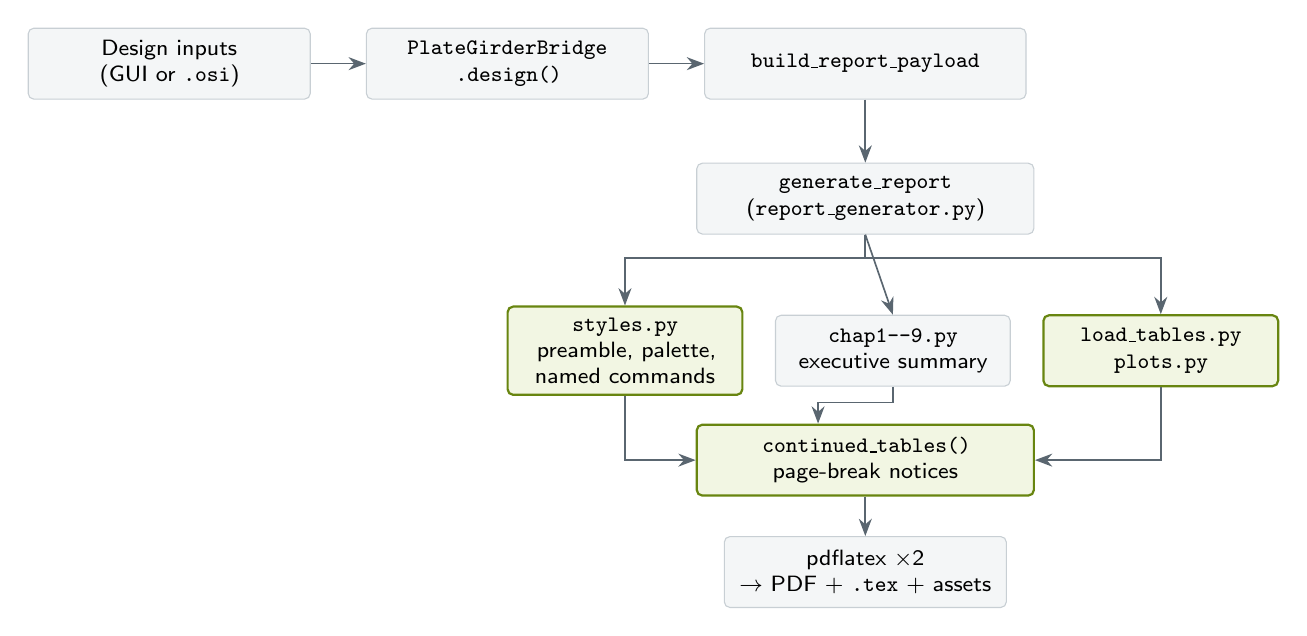
\begin{tikzpicture}[
  node distance=5mm and 7mm,
  box/.style={draw=rule,fill=codebg,rounded corners=2pt,align=center,font=\sffamily\footnotesize,
              minimum height=9mm,inner sep=4pt,text width=#1},
  box/.default=33mm,
  new/.style={box=#1,draw=brand,line width=0.8pt,fill=brandlight!12},
  new/.default=33mm,
  arr/.style={-{Stealth[length=2.2mm]},color=muted,line width=0.6pt}]
\node[box] (in) {Design inputs\\(GUI or \code{.osi})};
\node[box,right=of in] (solve) {\code{PlateGirderBridge}\\\code{.design()}};
\node[box=38mm,right=of solve] (payload) {\code{build\_report\_payload}};
\node[box=40mm,below=8mm of payload] (gen) {\code{generate\_report}\\(\file{report\_generator.py})};
\node[new=27mm,below left=9mm and -6mm of gen] (styles) {\file{styles.py}\\preamble, palette,\\named commands};
\node[box=27mm,right=4mm of styles] (chap) {\file{chap1--9.py}\\executive summary};
\node[new=27mm,right=4mm of chap] (load) {\file{load\_tables.py}\\\file{plots.py}};
\node[new=40mm,below=24mm of gen] (cont) {\code{continued\_tables()}\\page-break notices};
\node[box,below=of cont] (tex) {pdflatex $\times$2\\$\rightarrow$ PDF + \code{.tex} + assets};
\draw[arr] (in) -- (solve);
\draw[arr] (solve) -- (payload);
\draw[arr] (payload) -- (gen);
\draw[arr] (gen.south) -- ++(0,-3mm) -| (styles.north);
\draw[arr] (gen.south) -- (chap.north);
\draw[arr] (gen.south) -- ++(0,-3mm) -| (load.north);
\draw[arr] (styles.south) |- (cont.west);
\draw[arr] (chap.south) -- ++(0,-2mm) -| ([xshift=-6mm]cont.north);
\draw[arr] (load.south) |- (cont.east);
\draw[arr] (cont) -- (tex);
\end{tikzpicture}
\caption{Report generation pipeline. Green outlines mark modules added in this work.}
\label{fig:pipeline}
\end{figure}

\begin{longtable}{@{}L{4.4cm} >{\raggedright\arraybackslash}p{\dimexpr\linewidth-4.4cm-2\tabcolsep}@{}}
\caption{Files Added or Changed}\label{tab:files}\\
\toprule
\thead \hd{File} & \hd{Change} \\
\midrule
\endfirsthead
\toprule
\thead \hd{File} & \hd{Change} \\
\midrule
\endhead
\midrule
\multicolumn{2}{r}{\footnotesize\itshape Continued on next page}\\
\endfoot
\bottomrule
\endlastfoot
\file{styles.py} (new) \under{core/reports/} & Preamble, geometry, palette, header and footer, named spacing and font
commands, chart theme, \code{report\_section} decorator, and \code{continued\_tables()}. \\
\file{plots.py} (new) \under{core/reports/} & Reads stored design results and BOQ totals, draws the UR and quantity charts
with Matplotlib's Agg canvas and returns PyLaTeX figures. \\
\file{load\_tables.py} (new) \under{core/reports/} & Builds Table~3.3 in the per-vehicle layout and Table~3.4, and
interprets the GUI checkbox values. \\
\file{report\_generator.py} \under{core/reports/} & Uses the shared preamble; applies \code{continued\_tables()}; keeps a
\code{<report>\_assets} folder so the saved \code{.tex} recompiles; reports success only when the current compiler run
produced the PDF; always emits Chapter~6 so Chapter~7 keeps its number; draws the Chapter~5 and~7 charts whether or not
\emph{Drawings} is ticked. \\
\file{chap1.py} to \file{chap9.py}, \file{executive\_summary.py} \under{core/reports/} & Long tables with repeated
headers; shared style commands; consistent header capitalisation. Chapter~3 uses the new load tables; Chapter~5 drops
tall \code{multirow} cells, embeds the UR chart and adds the missing summary rows; Chapter~7 embeds the quantity
charts. \\
\file{report\_utils.py} \under{core/reports/} & Single-pass LaTeX escaping, so backslashes are not escaped twice;
negative figure spacing removed. \\
\file{boq\_generator.py} \under{core/boq/} & Bracing chord quantities follow the top and bottom chord settings. \\
\file{template\_page.py}, \file{output\_dock.py} \under{desktop/ui/, desktop/ui/docks/} & \emph{File $\rightarrow$ Create
Design Report} goes through the same 3D-view and plot capture as the Output panel's \emph{Generate Report}. \\
\file{test\_reports.py} (new) \under{tests/unit/} & 35 report tests (Section~\ref{sec:tests}). \\
\file{scripts/} (new) \under{repository root} & \file{run\_design\_validation.py}, \file{generate\_validation\_report.py},
\file{report\_layout\_fixture.py}, \file{check\_environment.py}. \\
\file{pyproject.toml}, \file{requirements-\allowbreak{}reports.txt} \under{repository root} & Declare PyLaTeX and
Matplotlib, and a light install for the report tests. \\
\end{longtable}
{\footnotesize\color{muted}Directories are relative to \file{src/osdagbridge/} unless marked as the repository root.}

% ================================================================ 4 ===========
\section{Defects found and fixed}\label{sec:defects}

Three defects outside the six requirements were found while validating the reports. Each was fixed and covered by a
regression test.

\begin{table}[!htbp]
\caption{Defects Found and Fixed}
\small
\begin{tabularx}{\linewidth}{@{}L{2.9cm} Y Y Y@{}}
\toprule
\thead \hd{Defect} & \hd{Symptom} & \hd{Cause} & \hd{Fix} \\
\midrule
BOQ bracing chords & Bracing tonnage in Table~7.1 and Figure~7.1 too high when a chord is disabled &
\code{top\_chord\_enabled} and \code{bot\_chord\_enabled} were hardcoded to \code{True} in \file{boq\_generator.py} &
Read the chord settings recorded by the cross-bracing force calculation \\
Drawings missing from menu reports & Every figure a placeholder when the report was started from the File menu &
\emph{File $\rightarrow$ Create Design Report} opened the dialog without capturing the 3D views and plots &
Route the menu through the Output panel's capture step \\
Report crash with drawings & ``PDF could not be generated'' once drawings were captured &
The bracing dialog adds text entries (\code{ed\_type}, \code{ed\_bracing\_type}) to the bracing results at run time,
and the chart code expected only member results & Read only member results; ignore other entries \\
\bottomrule
\end{tabularx}
\end{table}

% ================================================================ 5 ===========
\section{Design decisions}

Table~\ref{tab:decisions} records the main design decisions and why they were taken.

\begin{table}[!htbp]
\caption{Main Design Decisions and Their Rationale}\label{tab:decisions}
\small
\begin{tabularx}{\linewidth}{@{}L{4.4cm} Y@{}}
\toprule
\thead \hd{Decision} & \hd{Reason} \\
\midrule
Explicit longtable heads written in place & The chapters already write raw LaTeX; this keeps the change reviewable and
avoids rewriting about 3{,}200 lines of chapter code as PyLaTeX objects \\
Page-break notices added by one function & No chapter needs to know about them, and every table, current or future, gets
the same treatment \\
Reserve footer space in the geometry & Removes the cause of the overlap for every page, instead of patching individual
pages \\
Charts use the same rules as the tables & The chart and the Section~5.5 table can never disagree; a test enforces it \\
N/A instead of zero for missing data & A zero-height bar would look like a passing check \\
Matplotlib Agg canvas, not \code{pyplot} & Reports are generated inside the Qt desktop app, where \code{pyplot} could
switch the global backend or touch GUI state \\
Vertical UR chart & Matches the task: UR on the y-axis with a horizontal line at 1.0 \\
No solver changes & The task is about presentation; engineering issues are reported for the maintainers
(Section~\ref{sec:limits}) \\
\bottomrule
\end{tabularx}
\end{table}

% ================================================================ 6 ===========
\needspace{38\baselineskip}
\section{Visual enhancements}

Besides the six requirements, the presentation changes in Table~\ref{tab:visual} were made.

\begin{table}[!htbp]
\caption{Presentation Changes Beyond the Six Requirements}\label{tab:visual}
\small
\begin{tabularx}{\linewidth}{@{}L{3.6cm} Y Y@{}}
\toprule
\thead \hd{Item} & \hd{Before} & \hd{After} \\
\midrule
Table headers & ``parameter / value'' in 26 tables & ``Parameter / Value'' throughout; new tables add a Unit column \\
Per-girder tables (Chapter~5) & First column heading blank & ``Girder'' \\
Tables split across pages & No closing rule, no indication of continuation & Closing rule and ``continued'' notices \\
Page header & Stray ``\textbar'' when the job number is empty & Separator only when there is a job number \\
Chapter numbering & Material Take-off became Chapter~6 when drawings were not selected & Chapter~6 kept with a short
note, so Material Take-off is always Chapter~7 \\
Section~5.5 summary & Some governing checks missing & Deck SLS stress, deck minimum reinforcement and end-diaphragm
slenderness rows added \\
Bracing-type end diaphragm & Rows labelled Moment / Shear & Compression / Tension / Slenderness (``as bracing'') \\
Saved \code{.tex} & Referenced deleted temporary images & Images kept beside it; recompiles as delivered \\
\bottomrule
\end{tabularx}
\end{table}

% ================================================================ 7 ===========
\section{Validation}\label{sec:validation}

This section describes the design case, how the three reports were produced, the results and the regression tests.

\subsection{Design case and method}

All reports in this document come from the design case in Table~\ref{tab:case}.

\begin{table}[!htbp]
\caption{Validation Design Case}\label{tab:case}
\small
\begin{tabularx}{\linewidth}{@{}L{4.4cm} Y@{}}
\toprule
\thead \hd{Input} & \hd{Value} \\
\midrule
Span / carriageway width & 20\,m / 7.5\,m, no median \\
Footways                 & both sides, 1.5\,m (overall width 12.15\,m) \\
Skew                     & 0\textdegree \\
Location                 & Maharashtra (wind and seismic data from the project-location database) \\
Vehicles                 & all eight IRC classes selected \\
Design mode / materials  & Optimized / application defaults (E\,350A steel, M40 deck) \\
Input files              & \file{validation/design/inputs.json} and the equivalent \file{Report\_Validation.osi} \\
\bottomrule
\end{tabularx}
\end{table}

\file{scripts/run\_design\_validation.py} runs the real solver (\code{PlateGirderBridge.design()}) and saves its result,
with the Chapter~4 load-case and reaction summaries, exactly as \code{generate\_design\_report} passes them when
\emph{Generate Report} is clicked; running the design twice gives identical results.
\file{scripts/generate\_validation\_report.py} then builds both PDFs from that one result through the same
\code{build\_report\_payload} and \code{generate\_report} calls the GUI uses: \file{Report\_Before} with the unchanged
upstream report code (\code{d74f56d}) and \file{Report\_After} with this branch. \file{Report\_After\_GUI} was produced
in the desktop app (Design, then \emph{File $\rightarrow$ Create Design Report}) and includes the CAD drawings and
analysis plots.

\subsection{Results}

Table~\ref{tab:key} summarises the comparison. The original generator runs pdfTeX in non-stop mode and keeps the PDF
despite the errors, so \file{Report\_Before.pdf} is the real original output, errors included. Every numeric value in
\file{Report\_Before.pdf} also appears in \file{Report\_After.pdf}, and spot checks against the solver output (girder
moment, fatigue stress, SLS stress, LTB, governing UR) match in both.

\subsection{Test suite}\label{sec:tests}

Table~\ref{tab:tests} groups the report tests by area; Table~\ref{tab:env} lists the environment they ran in.

\begin{table}[!htbp]
\caption{Report Regression Tests in \file{tests/unit/test\_reports.py}}\label{tab:tests}
\small
\begin{tabularx}{\linewidth}{@{}L{3.6cm} Y C{1.2cm}@{}}
\toprule
\thead \hd{Area} & \hd{What is checked} & \hd{Tests} \\
\midrule
Tables and styles & Header repetition and page-break notices in every table; footer space reserved; palette and page
header; no hardcoded formatting outside \file{styles.py} & 5 \\
Live loads & GUI checkbox values; vehicle and footway selection; automatic footway pressure; Table~3.3 layout and values & 10 \\
Utilization chart & Ratios from all members and load cases; bracing slenderness; end-diaphragm rule; agreement with the
Section~5.5 table on the real design; live bracing entries; invalid data never drawn as zero & 12 \\
Quantities & Units and partial sums; chord settings in the BOQ; chart files created and embedded & 3 \\
Generator and GUI & Assets and stale-PDF handling; missing compiler; charts without drawings; Chapter~6 placeholder; File
menu capture & 5 \\
\midrule
\multicolumn{2}{@{}l}{\textbf{Total report tests} (the suite also has 5 existing tests; 40 in all)} & \textbf{35} \\
\bottomrule
\end{tabularx}
\end{table}

\begin{table}[!htbp]
\caption{Test and Build Environment}\label{tab:env}
\small
\begin{tabularx}{\linewidth}{@{}L{4.4cm} Y@{}}
\toprule
\thead \hd{Component} & \hd{Version} \\
\midrule
Operating system & Windows 11 \\
Python           & 3.12.16 (application environment from \file{environment.yml}) \\
PyLaTeX / Matplotlib & 1.4.2 / 3.10.9 \\
LaTeX            & pdfTeX 1.40.28 (TeX Live 2025, bundled with Osdag) \\
Result           & 40 passed; the GUI test is skipped where PySide6 is not installed \\
\bottomrule
\end{tabularx}
\end{table}

% ================================================================ 8 ===========
\section{Known limitations (upstream, not changed here)}\label{sec:limits}

These are in the structural analysis rather than the report layer. Fixing them would change design results, so they
are left for maintainer review. The report shows the values as computed and explains each N/A in its notes.

\begin{table}[!htbp]
\caption{Limitations Visible in the Report}
\small
\begin{tabularx}{\linewidth}{@{}L{3.4cm} Y Y@{}}
\toprule
\thead \hd{Item} & \hd{Seen in the report} & \hd{Cause} \\
\midrule
Braking force & N/A in Table~3.3 & No braking load case in the analysis; \code{IRC6\_2017.cl\_211\_2\_braking\_force}
raises \code{UnboundLocalError} for every lane count \\
Vehicle selection & Table~3.3 lists every selected vehicle & The grillage analysis takes Class~A and Class~70R
(wheeled) from IRC~6 Table~6A and applies the Cl.~208.3 impact factor to every vehicle case \\
Deflection & Sections 4 and 5.1: 28.81\,mm live load, 70.42\,mm total (FAIL); Section~5.5: 11.03\,mm and 24.50\,mm &
The analysis tables and the design module's girder checks use different values; the original report shows the same \\
Values not produced & N/A for centrifugal force and end-diaphragm tonnage; empty wind and earthquake rows &
Not calculated by the current code \\
Drawings & Placeholders in the script-made reports & Need the GUI's CAD capture; \file{Report\_After\_GUI.pdf} has them \\
Failing check & Fatigue UR 2.56 for this design & Kept to show the failing state of the chart and table \\
\bottomrule
\end{tabularx}
\end{table}

% ================================================================ 9 ===========
\needspace{20\baselineskip}
\section{Deliverables}

Table~\ref{tab:deliv} lists the submitted files.

\begin{table}[!htbp]
\caption{Submitted Files (Paths Relative to the Repository Root)}\label{tab:deliv}
\small
\begin{tabularx}{\linewidth}{@{}L{6.4cm} Y@{}}
\toprule
\thead \hd{File} & \hd{Description} \\
\midrule
\file{validation\pathsep design\pathsep Report\_Before.pdf} & Original output, unchanged upstream code \\
\file{validation\pathsep design\pathsep Report\_After.pdf}  & Refactored output, same design result \\
\file{validation\pathsep design\pathsep Report\_After\_GUI.pdf} & Refactored output from the desktop app, with drawings \\
\file{validation\pathsep design\pathsep *.tex} and \file{*\_assets\pathsep} & LaTeX sources and images; each report recompiles \\
\file{validation\pathsep design\pathsep Report\_Validation.osi} & Design inputs, loadable in the application \\
\file{docs\pathsep FOSSEE\_TECHNICAL\_CHANGES.pdf} & This document (source: \file{.tex}) \\
\file{src\pathsep osdagbridge\pathsep ...}, \file{tests\pathsep unit\pathsep test\_reports.py} & Source changes and tests \\
\bottomrule
\end{tabularx}
\end{table}

% ================================================================ 10 ==========
\needspace{18\baselineskip}
\section{Reproducing}

\needspace{15\baselineskip}
\begin{lstlisting}
conda env create -f environment.yml
conda activate osdagbridge-env
pip install -r requirements-reports.txt      # report tests only
pytest tests -q

# from the repository root, with PYTHONPATH=src
python scripts/run_design_validation.py      # writes inputs.json and outputs.json
python scripts/generate_validation_report.py # Report_After.pdf
# Report_Before: upstream d74f56d src first on PYTHONPATH, then
python scripts/generate_validation_report.py --baseline
\end{lstlisting}

Windows installation notes are in \file{docs/LOCAL\_ENVIRONMENT.md}.

\end{document}
